\section{گام چهارم: ارزیابی نهایی و تحلیل ماتریس درهم‌ریختگی}

پس از پایان فرآیند آموزش، بهترین مدل ذخیره‌شده (بر اساس کمترین خطای اعتبارسنجی) بارگذاری شد و روی مجموعه‌ی آزمون \lr{(Test Set)} که مدل تا به حال آن را ندیده بود، مورد ارزیابی قرار گرفت. 

\subsection{معیارهای ارزیابی و گزارش دسته‌بندی}
با توجه به اینکه مجموعه داده‌ی \lr{FER2013} دارای عدم تعادل کلاسی \lr{(Class Imbalance)} شدیدی است، اتکا به معیار «دقت کل» \lr{(Accuracy)} به تنهایی گمراه‌کننده خواهد بود. بنابراین، معیارهای \lr{Precision}، \lr{Recall} و \lr{F1-score} برای هر کلاس به‌صورت مجزا محاسبه شدند. همچنین معیار \lr{Macro F1-score} که میانگین بدون وزن این معیارهاست و ارزش یکسانی برای کلاس‌های اقلیت و اکثریت قائل می‌شود، برابر با \lr{0.33} به دست آمد.

برای جلوگیری از خطاهای رندرینگ جداول، نتایج ارزیابی تفکیک‌شده برای هر کلاس به شکل زیر گزارش می‌شود:

\begin{itemize}
    \item \textbf{خشم \lr{(Angry)}:} \\
    تعداد نمونه: \lr{491} | \lr{Precision: 0.32} | \lr{Recall: 0.21} | \lr{F1-score: 0.25}
    
    \item \textbf{انزجار \lr{(Disgust)}:} \\
    تعداد نمونه: \lr{55} | \lr{Precision: 0.33} | \lr{Recall: 0.02} | \lr{F1-score: 0.03}
    
    \item \textbf{ترس \lr{(Fear)}:} \\
    تعداد نمونه: \lr{528} | \lr{Precision: 0.27} | \lr{Recall: 0.21} | \lr{F1-score: 0.24}
    
    \item \textbf{شادی \lr{(Happy)}:} \\
    تعداد نمونه: \lr{879} | \lr{Precision: 0.45} | \lr{Recall: 0.78} | \lr{F1-score: 0.57}
    
    \item \textbf{غم \lr{(Sad)}:} \\
    تعداد نمونه: \lr{594} | \lr{Precision: 0.33} | \lr{Recall: 0.29} | \lr{F1-score: 0.31}
    
    \item \textbf{تعجب \lr{(Surprise)}:} \\
    تعداد نمونه: \lr{416} | \lr{Precision: 0.60} | \lr{Recall: 0.48} | \lr{F1-score: 0.53}
    
    \item \textbf{خنثی \lr{(Neutral)}:} \\
    تعداد نمونه: \lr{626} | \lr{Precision: 0.47} | \lr{Recall: 0.34} | \lr{F1-score: 0.39}
\end{itemize}

\subsection{تحلیل ماتریس درهم‌ریختگی \lr{(Confusion Matrix)}}
برای درک بهتر خطاهای طبقه‌بندی، ماتریس درهم‌ریختگی بر روی داده‌های آزمون رسم گردید (شکل \ref{fig:cm}).

\begin{figure}[h!]
    \centering
    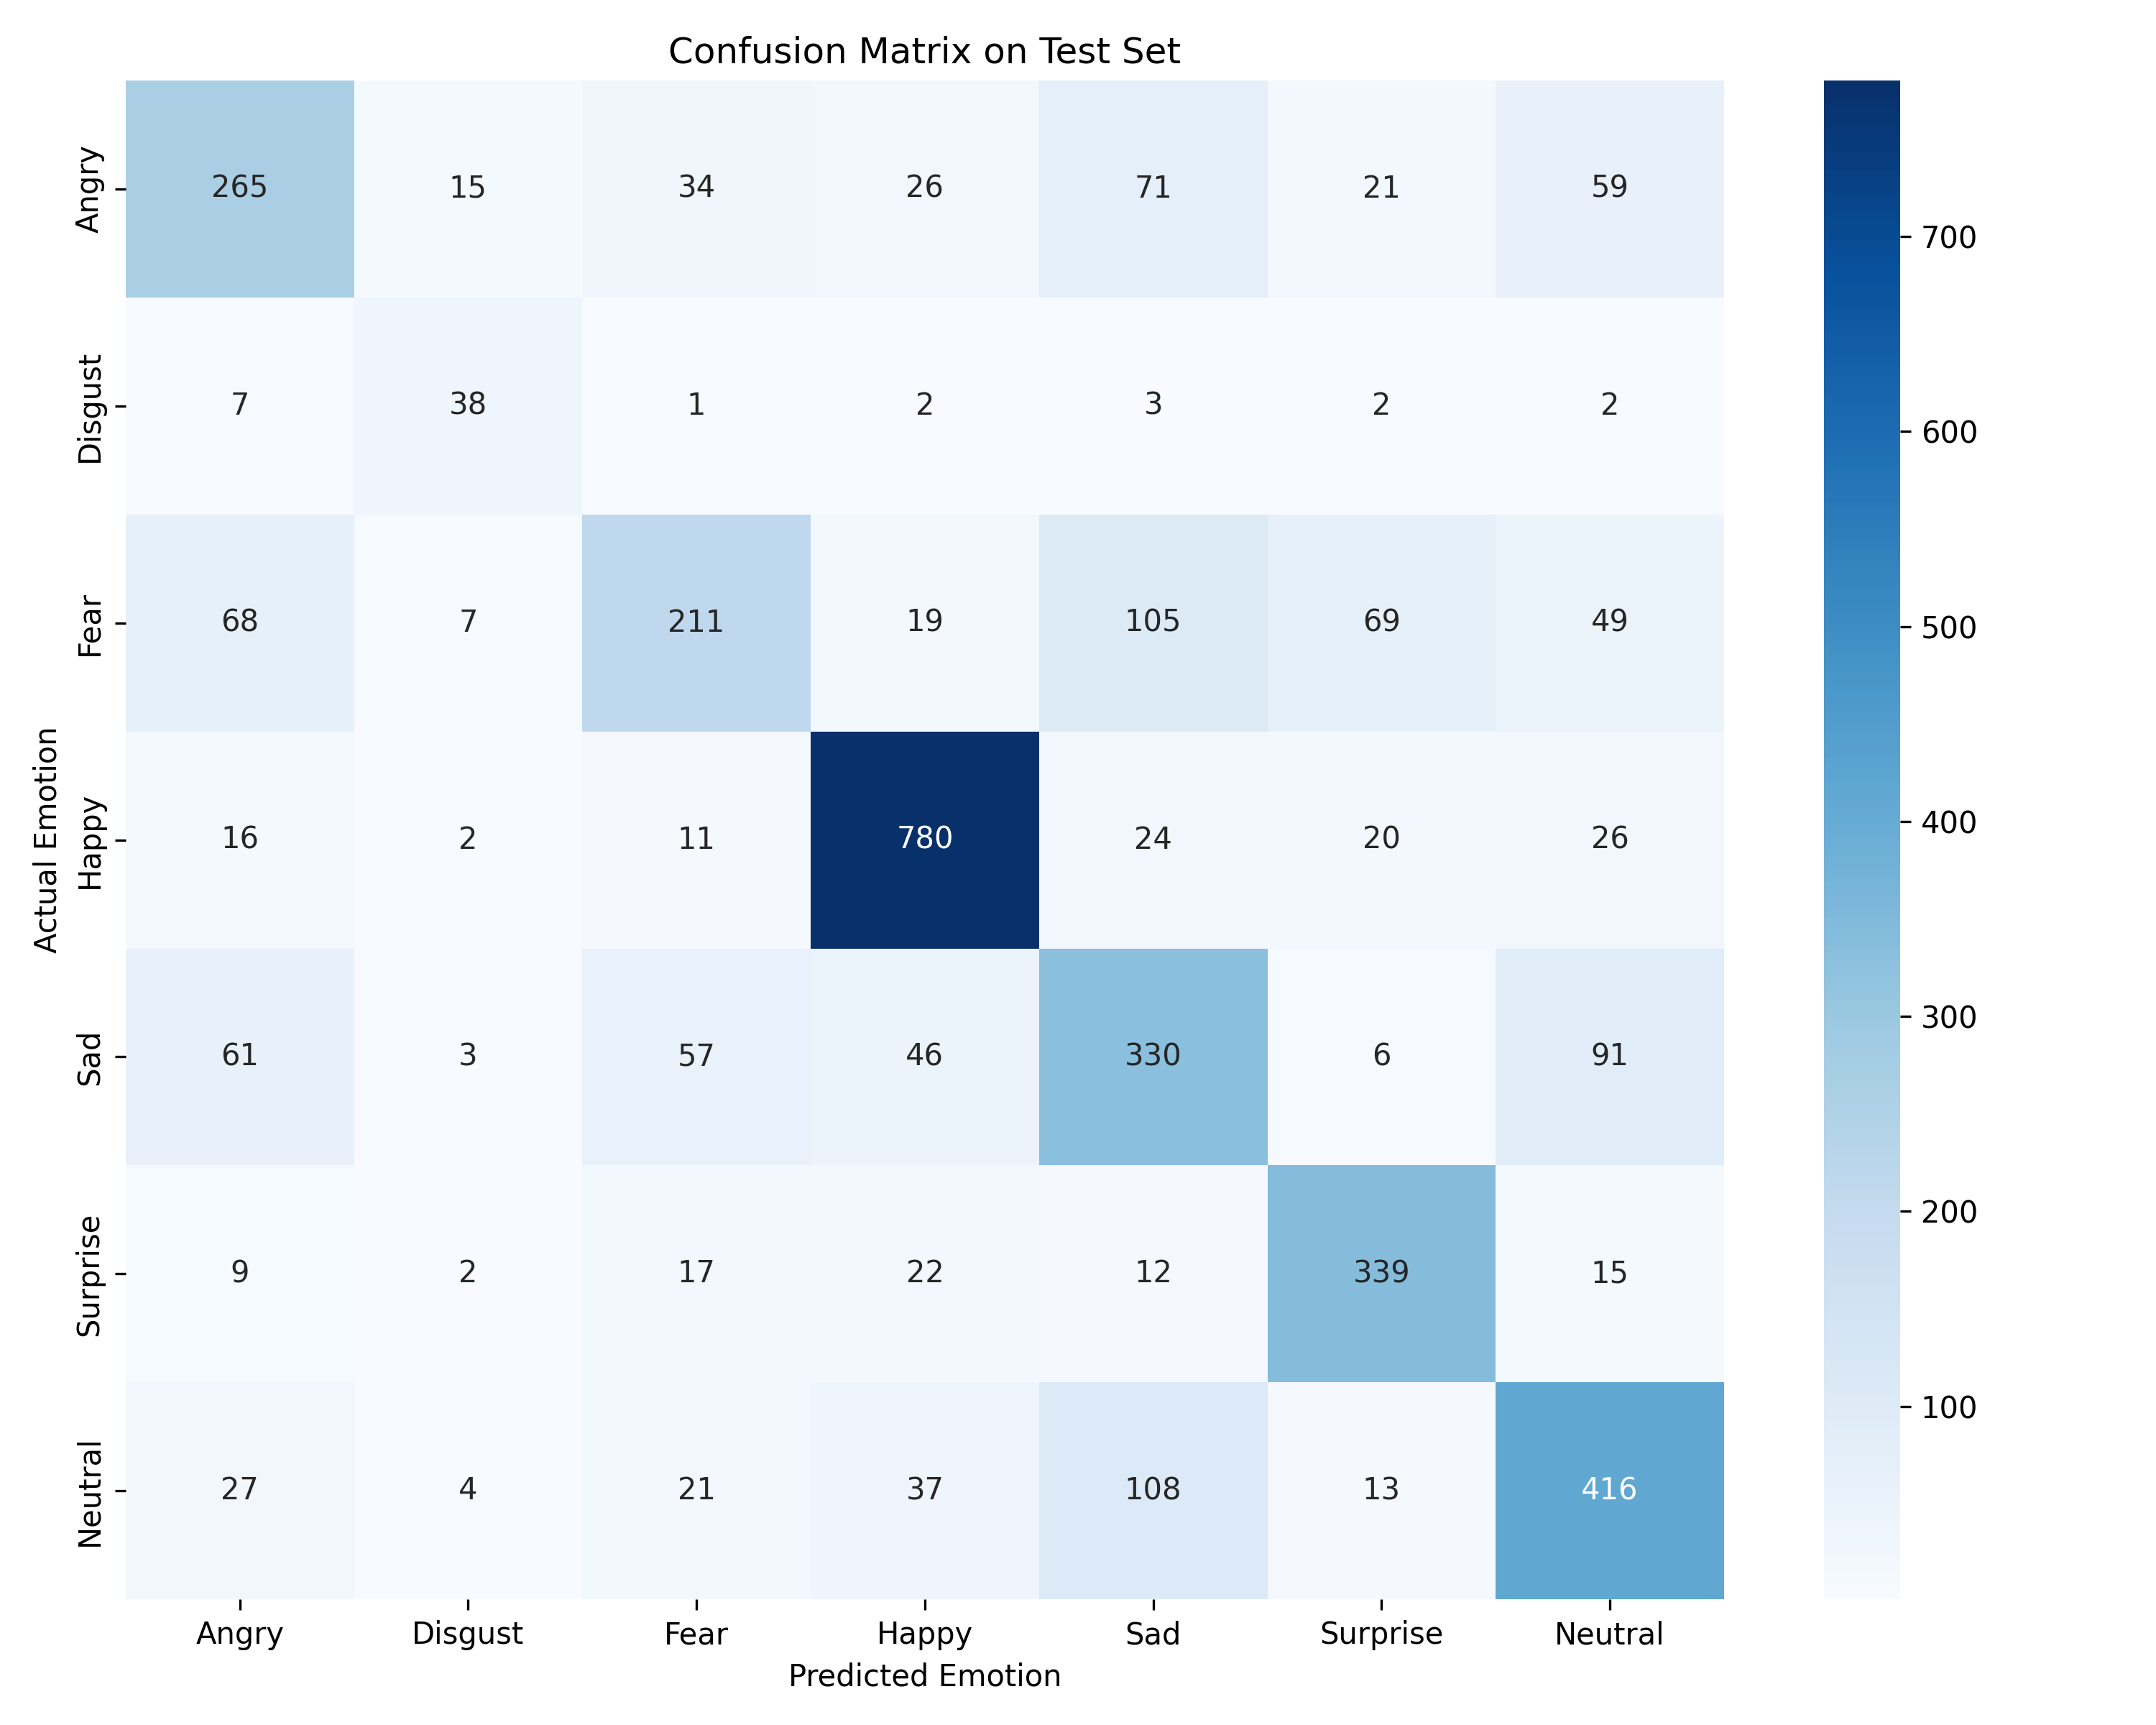
\includegraphics[width=0.85\textwidth]{images/confusion_matrix.png}
    \caption{ماتریس درهم‌ریختگی مدل یادگیری انتقالی روی مجموعه‌ی آزمون}
    \label{fig:cm}
\end{figure}

\subsubsection*{پاسخ به پرسش‌های تحلیلی:}
بر اساس ماتریس تولید شده، تحلیل خطاهای شبکه به شرح زیر است:
\begin{enumerate}
    \item \textbf{موفق‌ترین کلاس:} احساس شادی \lr{(Happy)} با تشخیص صحیح \lr{690} نمونه از \lr{879} نمونه (معادل \lr{Recall 78\%})، موفق‌ترین کلاس شبکه بوده است.
    \item \textbf{بیشترین خطا:} کلاس انزجار \lr{(Disgust)} بدترین عملکرد را داشته است؛ به‌طوری‌که تقریباً هیچ‌کدام از نمونه‌های آن به درستی تشخیص داده نشده‌اند.
    \item \textbf{بیشترین تداخل \lr{(Confusion)}:} بررسی ماتریس نشان می‌دهد که کلاس‌های خنثی \lr{(Neutral)} و غم \lr{(Sad)} به‌شدت با کلاس شادی \lr{(Happy)} اشتباه گرفته شده‌اند (به ترتیب \lr{205} و \lr{202} تشخیص اشتباه به عنوان \lr{Happy}).
    \item \textbf{علت تداخل و خطاها:} دو دلیل اصلی برای این رفتار وجود دارد. نخست \textbf{عدم تعادل شدید داده‌ها} است؛ کلاس \lr{Happy} با \lr{879} نمونه بر مجموعه غالب است، در حالی که کلاس \lr{Disgust} تنها \lr{55} نمونه دارد، لذا مدل سوگیری \lr{(Bias)} شدیدی به سمت پیش‌بینی کلاس اکثریت پیدا کرده است. دوم اینکه در روش یادگیری انتقالی پایه، لایه‌های استخراج ویژگی فریز شده‌اند؛ این لایه‌ها که روی اشیاء آموزش دیده‌اند، تغییرات ظریف عضلات صورت در احساساتی مانند غم یا ترس را به خوبی درک نمی‌کنند و صرفاً به دنبال ویژگی‌های برجسته‌تری مانند باز بودن دهان (که در شادی و تعجب مشترک است) می‌گردند.
\end{enumerate}